% \begin{frame}[noframenumbering]{Perspectives: Knowledge Graph}

%     \vspace{-1em}
%         \begin{center}
%             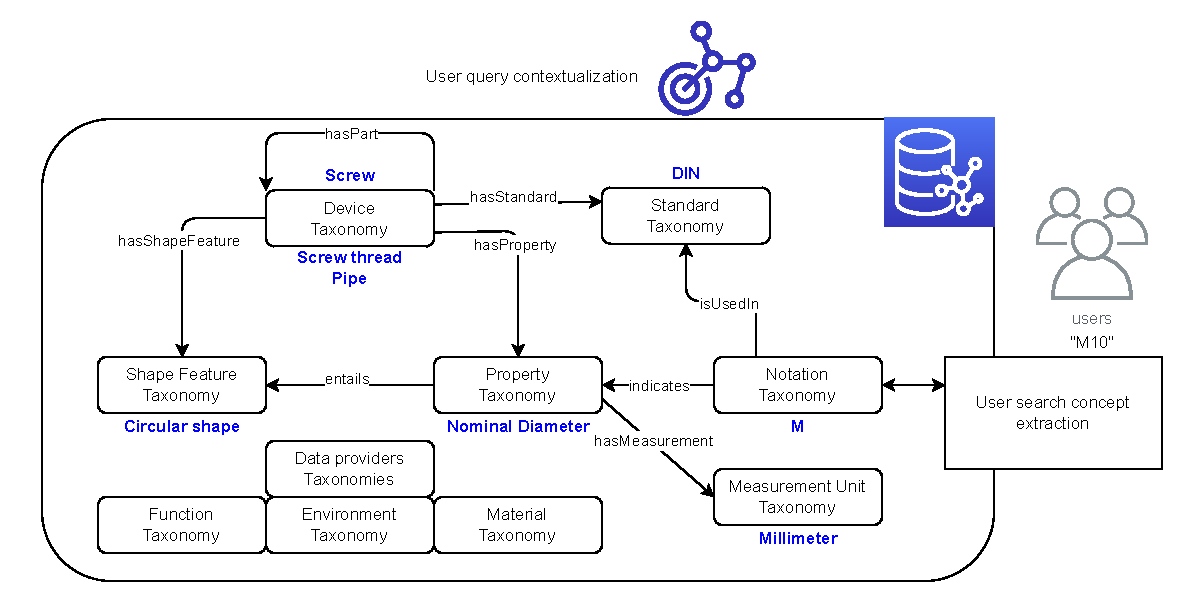
\includegraphics[scale=0.55]{images/semantic_search_example.pdf} 
%         \end{center}

% \end{frame}

\begin{frame}[noframenumbering]{Semantic Web Knowledge Graph}
    
        \begin{center}
            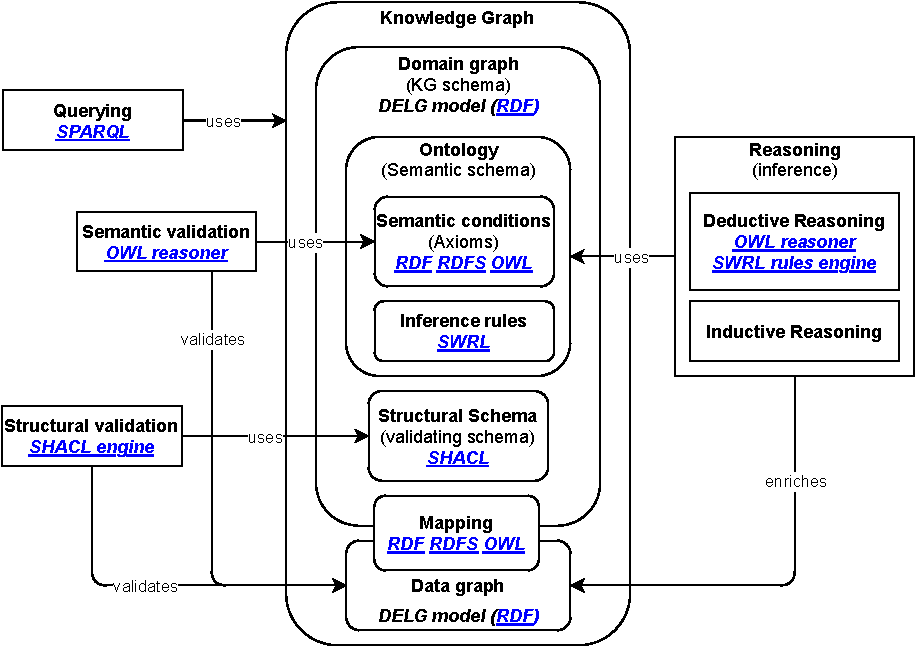
\includegraphics[scale=0.6]{images/kg-def-technos.pdf} 
        \end{center}

\end{frame}

% \begin{frame}{Online OWL reasoning-based approach}

%     An approach focusing on OWL.
    
%     \begin{itemize}
%         \item An Information Retrieval ontology.
%         \item Push knowledge closer to the data.
%         \item Model domain knowledge as linked sets of taxonomies. 
%     \end{itemize}

% \end{frame}

\begin{frame}[noframenumbering]{Knowledge modelling}

        \begin{center}
            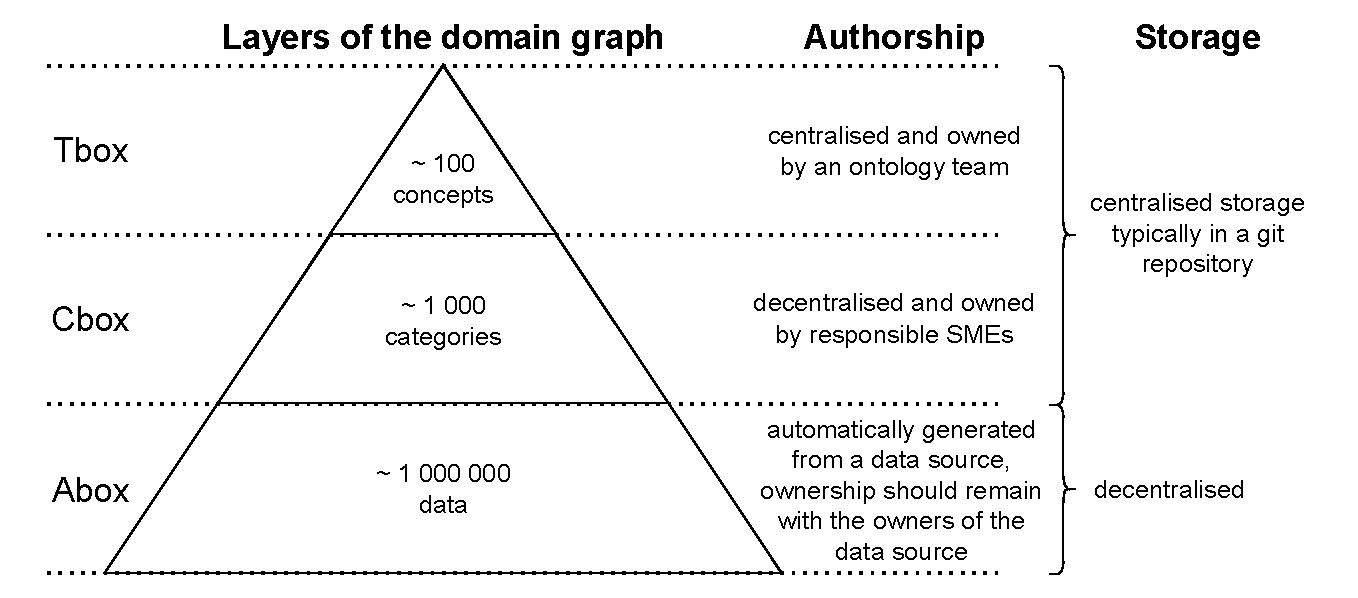
\includegraphics[scale=0.5]{images/TboxAboxCboxLayers.pdf} 
        \end{center}

\end{frame}

% \begin{frame}{Information Retrieval Ontology}

%     Competency questions:
%     \begin{itemize}
%         \item CQ1 What are the categories in the user search?
%         \item CQ2 What are the documents relevant to a search?
%         \item CQ3 What categories are enabled to refine the search?
%     \end{itemize}

%     7 classes:
%     \begin{itemize}
%         \item \emph{Candidate Document} subclass of \emph{Document} 
%         \item \emph{Selected Category} and \emph{Enabled Category} subclasses of \emph{Category}
%         \item \emph{Search Context} subclass of \emph{Search}
%     \end{itemize}

%     6 Object properties:
%     \begin{itemize}
%         \item \emph{categorises} inverse of \emph{categorised By}
%         \item \emph{has Search Category} subproperty of \emph{enables Category}
%         \item \emph{has Direct Subcategory} subproperty of \emph{has Subcategory}
%     \end{itemize}

% \end{frame}

% \begin{frame}{Pizza ontology}

%     Pizza ontology:
%     \begin{itemize}
%         \item Well-knowledge ontology built to introduce RDF/RDFS/OWL with examples (and even SHACL)
%         \item Simple ontology with class hierarchies of:
%         \begin{itemize}
%             \item Pizzas (has topping, has base)
%             \item Pizza bases
%             \item Pizza Toppings
%         \end{itemize} 
%     \end{itemize}

%     \begin{itemize}
%         \item We use the Pizza ontology for demonstration in interest of time constraints 
%     \end{itemize}

% \end{frame}

% \begin{frame}{Pizza ontology Knowledge Graph}

%     \begin{figure} [H]
%         \begin{center}
%             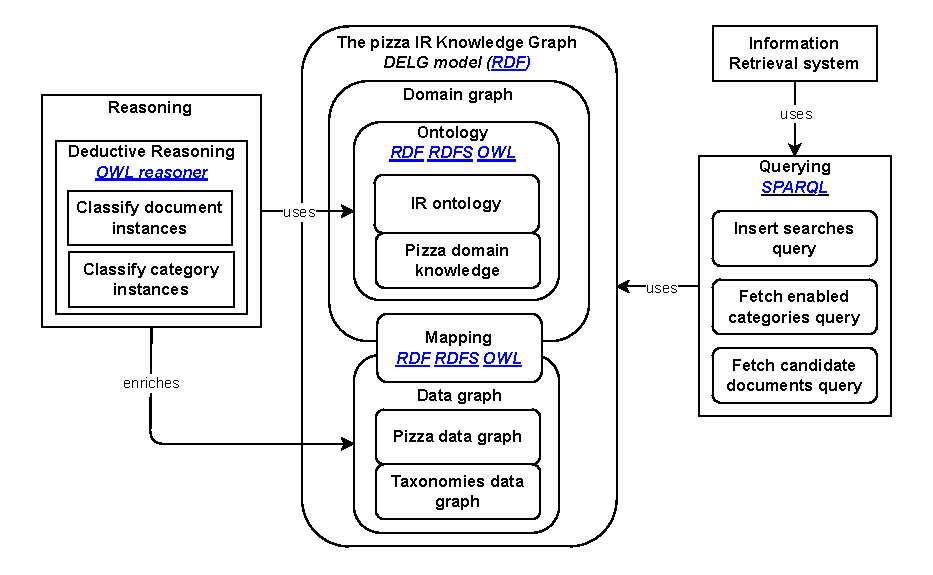
\includegraphics[scale=0.6]{images/pizza-demo-kg.pdf} 
%             \caption{Pizza ontology Knowledge Graph} 
%         \end{center}
%     \end{figure}
% \end{frame}


\begin{frame}[noframenumbering]{OWL reasoning-based Information Retrieval}

        \begin{center}
            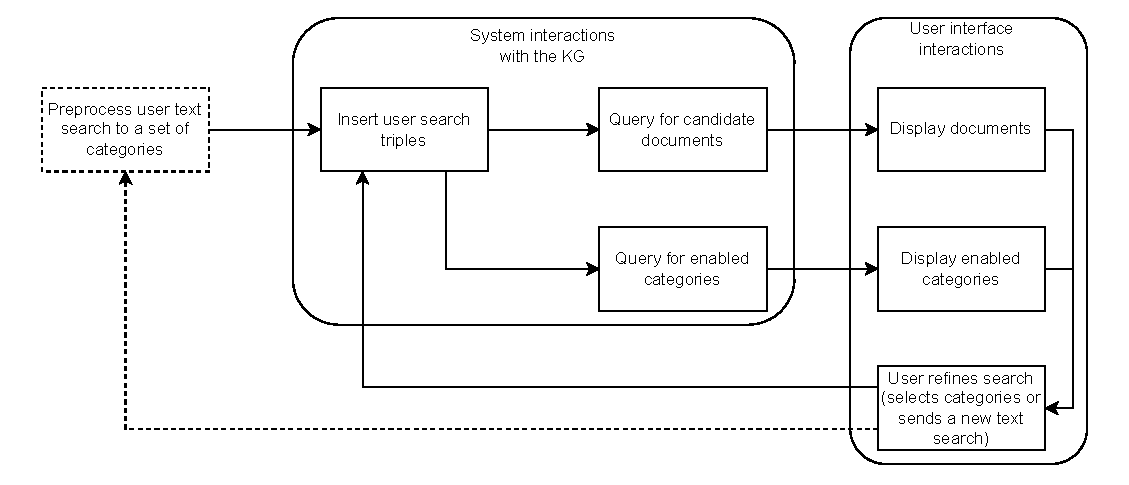
\includegraphics[scale=0.6]{images/ir-onto-search-process.pdf} 
        \end{center}

\end{frame}

\begin{frame}[noframenumbering]{Ontology Learning Applied Framework}

        \begin{center}
            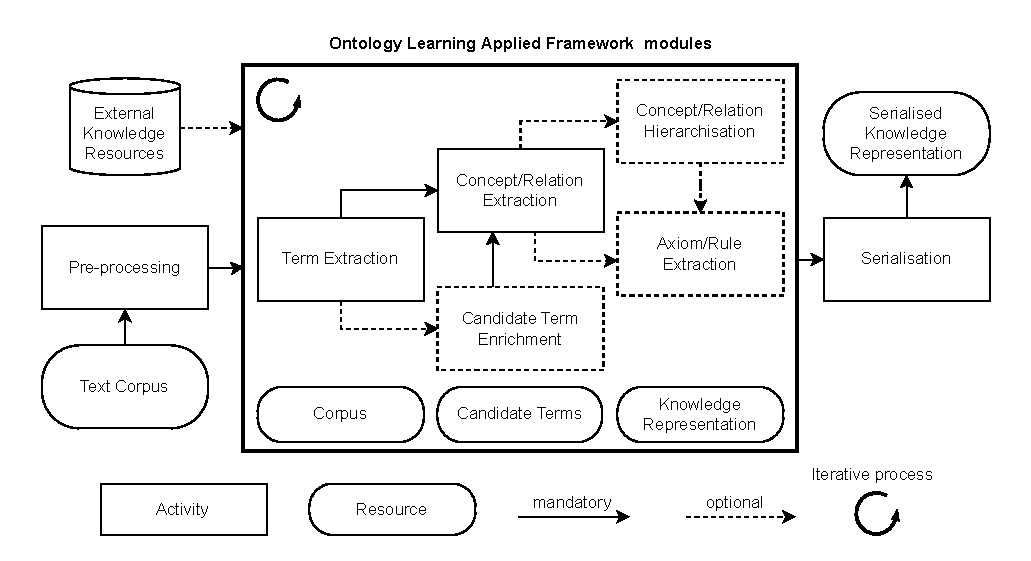
\includegraphics[scale=0.6]{images/olaf-modules.pdf} 
        \end{center}

\end{frame}

\begin{frame}[noframenumbering]{KG-based IR: Quantitative results}

        \begin{center}
        \small
        \begin{tabular}{ccc}
            \toprule
            {} &  \textbf{No results}  &  \textbf{\begin{tabular}[c]{@{}c@{}}Less than 400\\ results (non empty)\end{tabular}} \\
            \midrule
            \textbf{\begin{tabular}[c]{@{}c@{}}Text-based\\ system (baseline)\end{tabular}}              &     64.48\% &              35.44\% \\
            \textbf{\begin{tabular}[c]{@{}c@{}}Concept-based\\ system\end{tabular}}                      &     11.43\% &              \textbf{88.36\%} \\
            \textbf{\begin{tabular}[c]{@{}c@{}}KG-based system\\with search history\end{tabular}}      &     \textbf{8.10\%} &       51.59\% \\
            \bottomrule
        \end{tabular}
    \end{center}

\end{frame}